\documentclass[12pt]{article}

\usepackage{dsfont}
\usepackage{amsmath}
\usepackage{graphicx}
\usepackage[margin=1.00in]{geometry}

\usepackage{bm}
\newcommand{\m}[1]{\mathbf{\bm{#1}}}
\newcommand{\R}{I\hspace{-4.4pt}R}

\setlength\parindent{0pt}

\begin{document}


\begin{center}
\begin{huge}
Ozone in the Northeast United States
\end{huge}
\bigskip

Mickey Warner
\end{center}

\section{Abstract}

We fit a Gaussian process to ozone measurements at 107 locations in the northeastern United States. We found there to be linear trends in longitude and latitude as well as an interaction between the two. We attempted to fit a GP with a Mat{\'e}rn correlation and observation error, but this appeared to be unnecessary as our estimated implied there to be little to no covariance between observations.

\section{Introduction}

\subsection{Data}

The region we consider here comprises New England and a few states below along the east coast. Along this roughly 700 miles of east coast we have 107 measurement locations (Figure 1). Measurements are made up of yearly ozone averages (in parts per million) for 2015. Included in our data is the altitude (meters above sea level) at each location.

\begin{figure}[ht]
\begin{center}
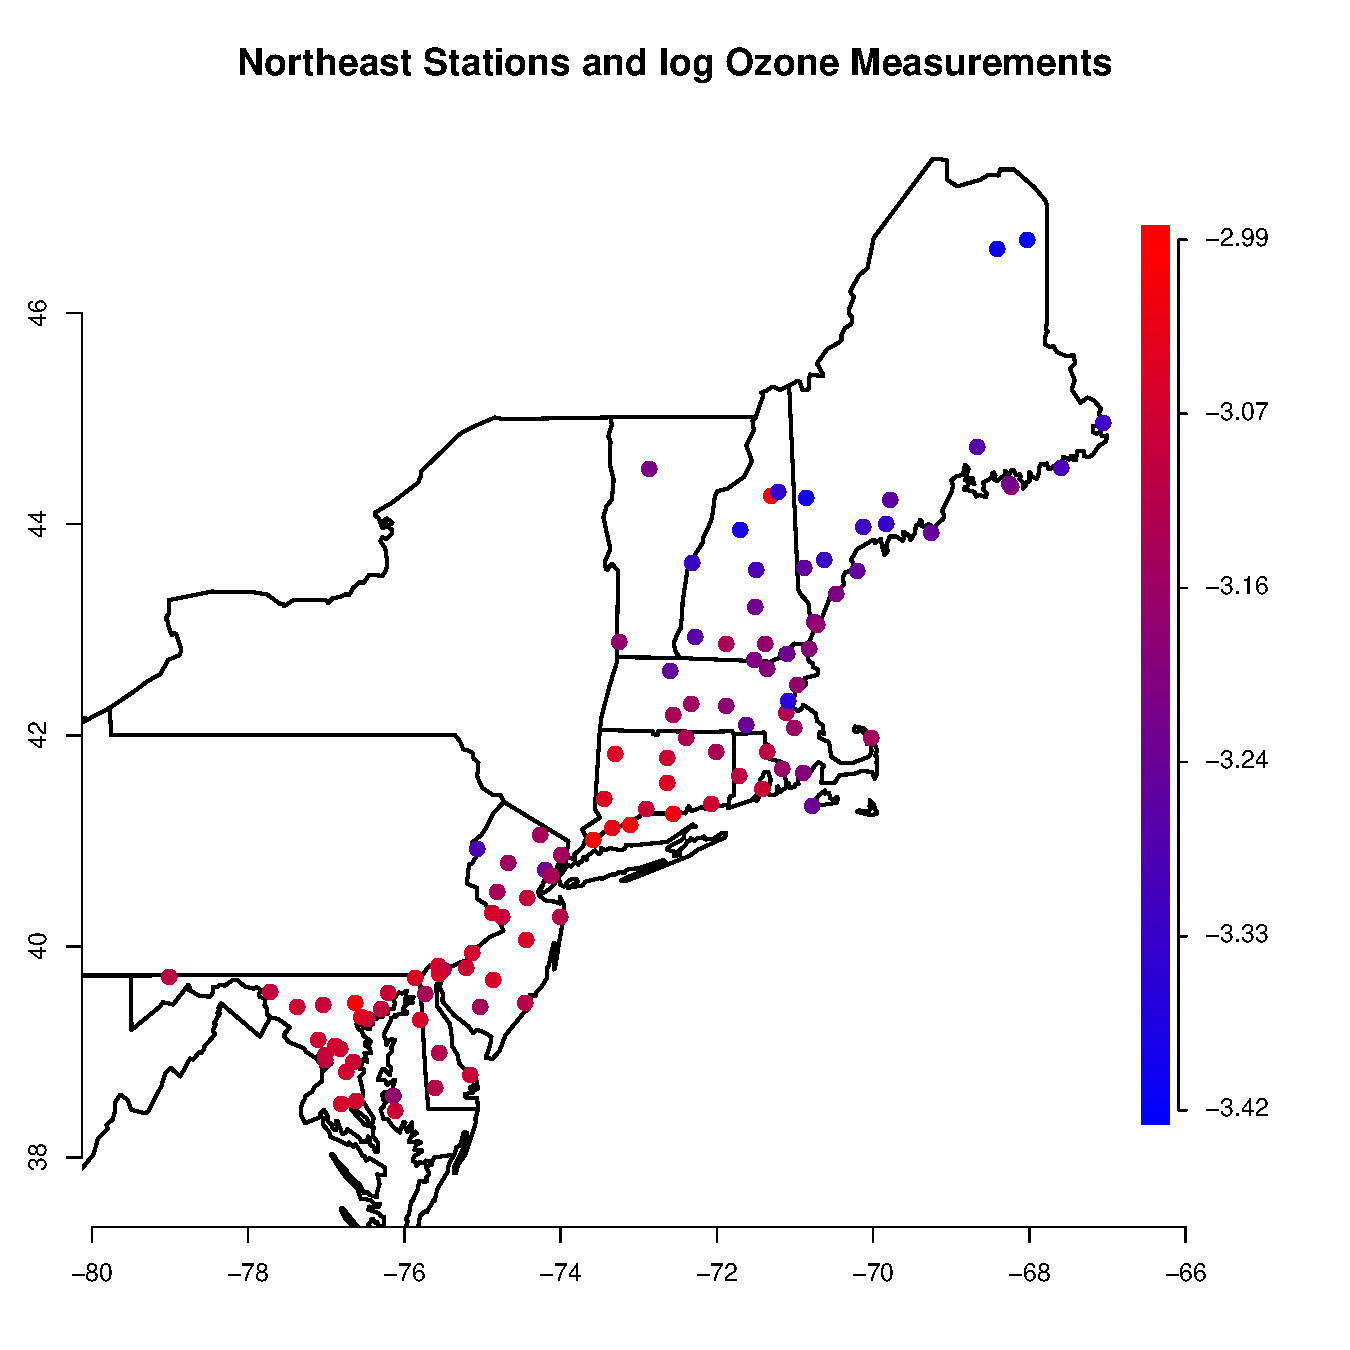
\includegraphics[scale=0.40]{figs/data.pdf}
\end{center}
\caption{Measurement locations of (log) ozone readings. Altitude not shown.}
\end{figure}

\subsection{Methods}

To analyze this data we will first explore possible trends. This can be achieved by fitting a classic linear regression with a variable selection method. We select variables from linear, quadratic, and interaction terms based on BIC. The chosen variables are then used as part of the mean in our GP. We will validate our model by looking at DIC.
\bigskip

In determining an appropriate correlation function, we can look at possibly anisotropies in the data by binning distances to estimate semivariances. Here, we will analyze the residuals from our chosen linear model. This is discussed more in section 3.
\bigskip

We fit our model on a training data set of 96 locations, leaving about 10\% out. If our model is a good fit, we should see reasonable predictions for the 11 locations from the test data set.

% DIC with all params: -227.2434
% DIC intercept: -239.0159

\section{Exploratory data analysis}

\subsection{Trends}

We explore possible trends in the data. Before we get to that, we make two adjustments to the data. First, we take the log of the ozone measurements to get closer to normality. Second, since we have a couple of observations with really high altitude, we add one to the altitude and take the log. This deals with the stations at 0 altitude and reduces the effect of possible leverage points.
\bigskip

Figure 2 hints at the possibility of some linear trends along some of the spatial dimensions. We fit a regression with linear and quadratic terms in each direction as well as interactions. Covariates are selected with a step-wise procedure with BIC as its selection criterion.

\begin{figure}[ht]
\begin{center}
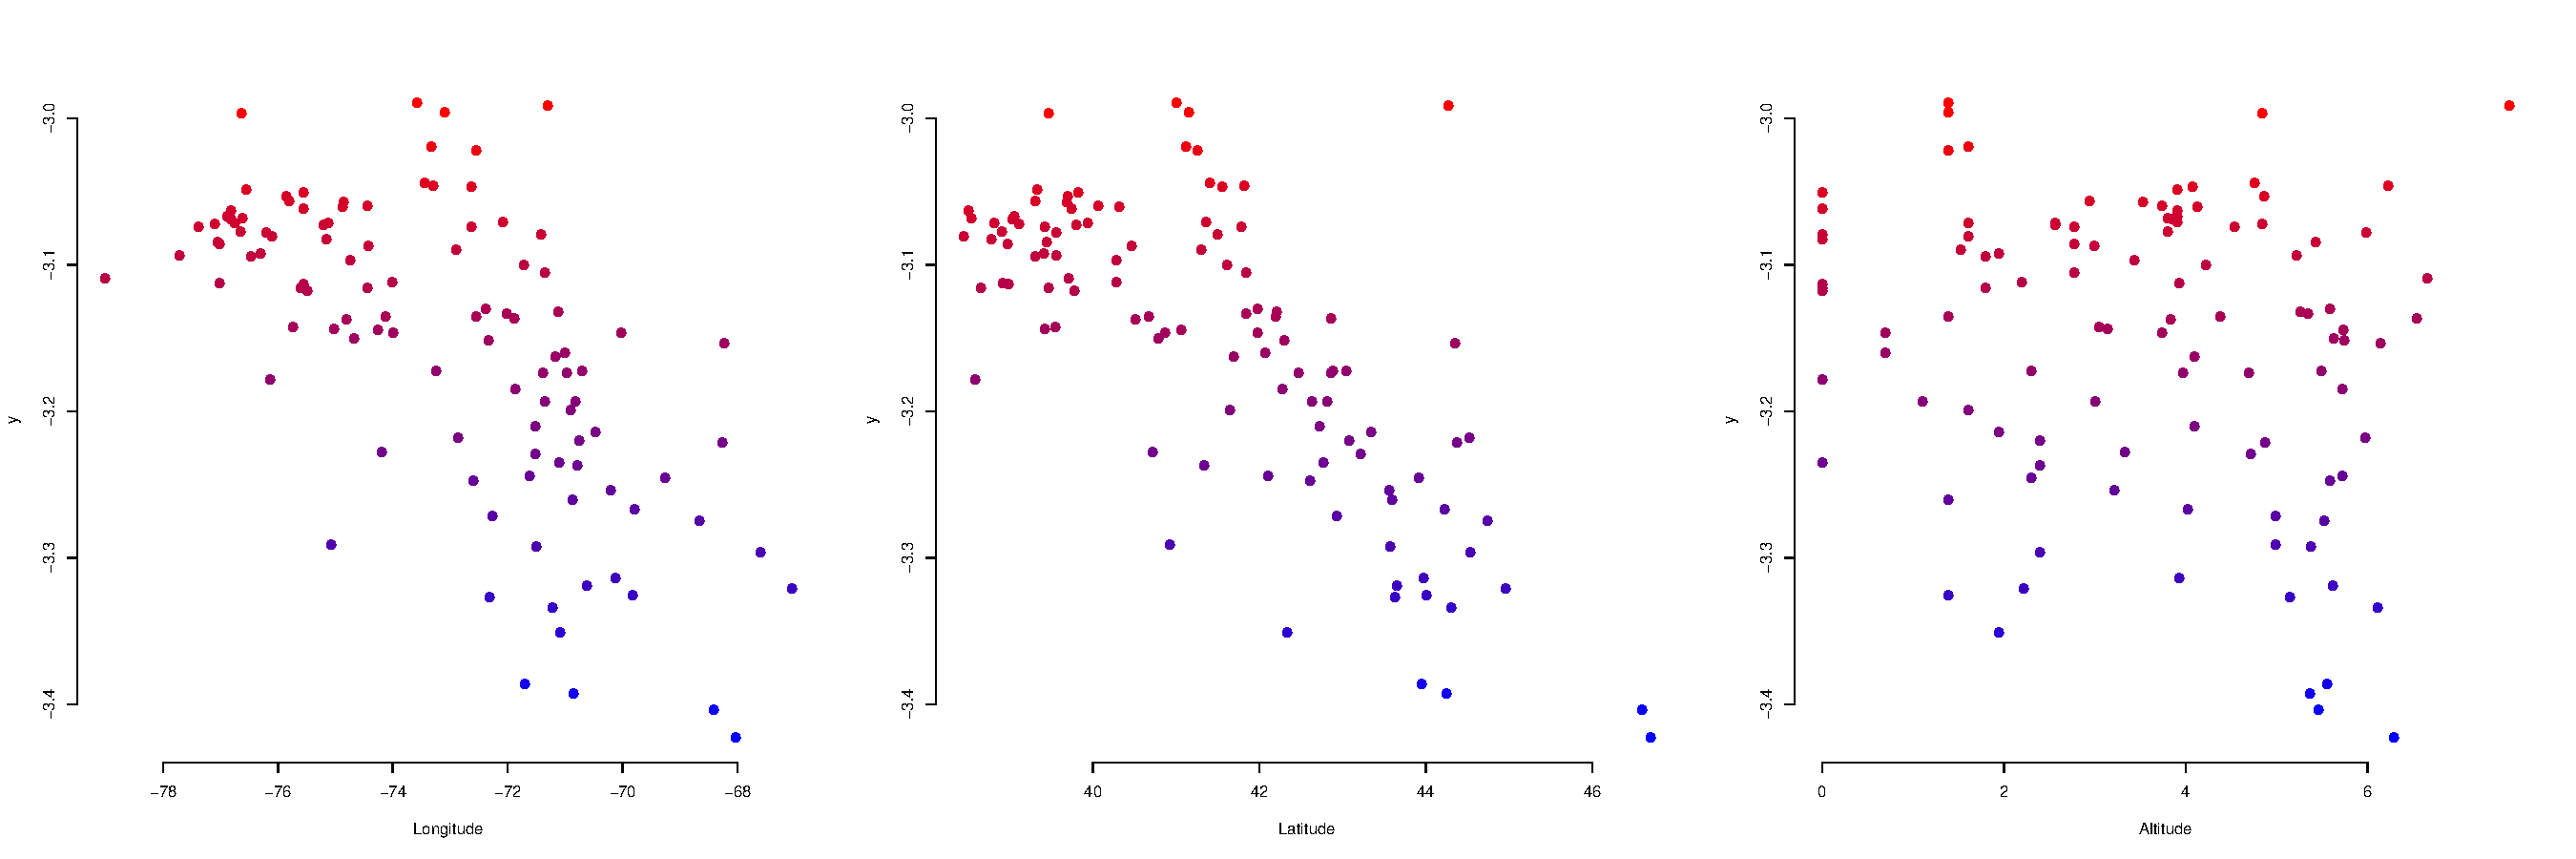
\includegraphics[scale=0.30]{figs/trend.pdf}
\end{center}
\caption{Each of three location types versus log ozone. The gray dots are the observed data, the black dots are the regression fit, and the liness represent the residuals.}
\end{figure}

The step-wise procedure selects an intercept, longitude, latitude, and an interaction between longitude and latitude. Altitude does not appear to have an influence on ozone.
\bigskip

\subsection{Semivariograms}

Using the residuals we compute a binned semivariogram from the data. We also look at the semivariogram in four directions to see if there is an anisotropy. The plots are given in Figure 3. We see from the right plot in Figure 3 that each direction produces more-or-less the same semivariogram, there is little difference between the curves. This suggests that we do not have enough evidence to believe there is anisotropy.

\begin{figure}[ht]
\begin{center}
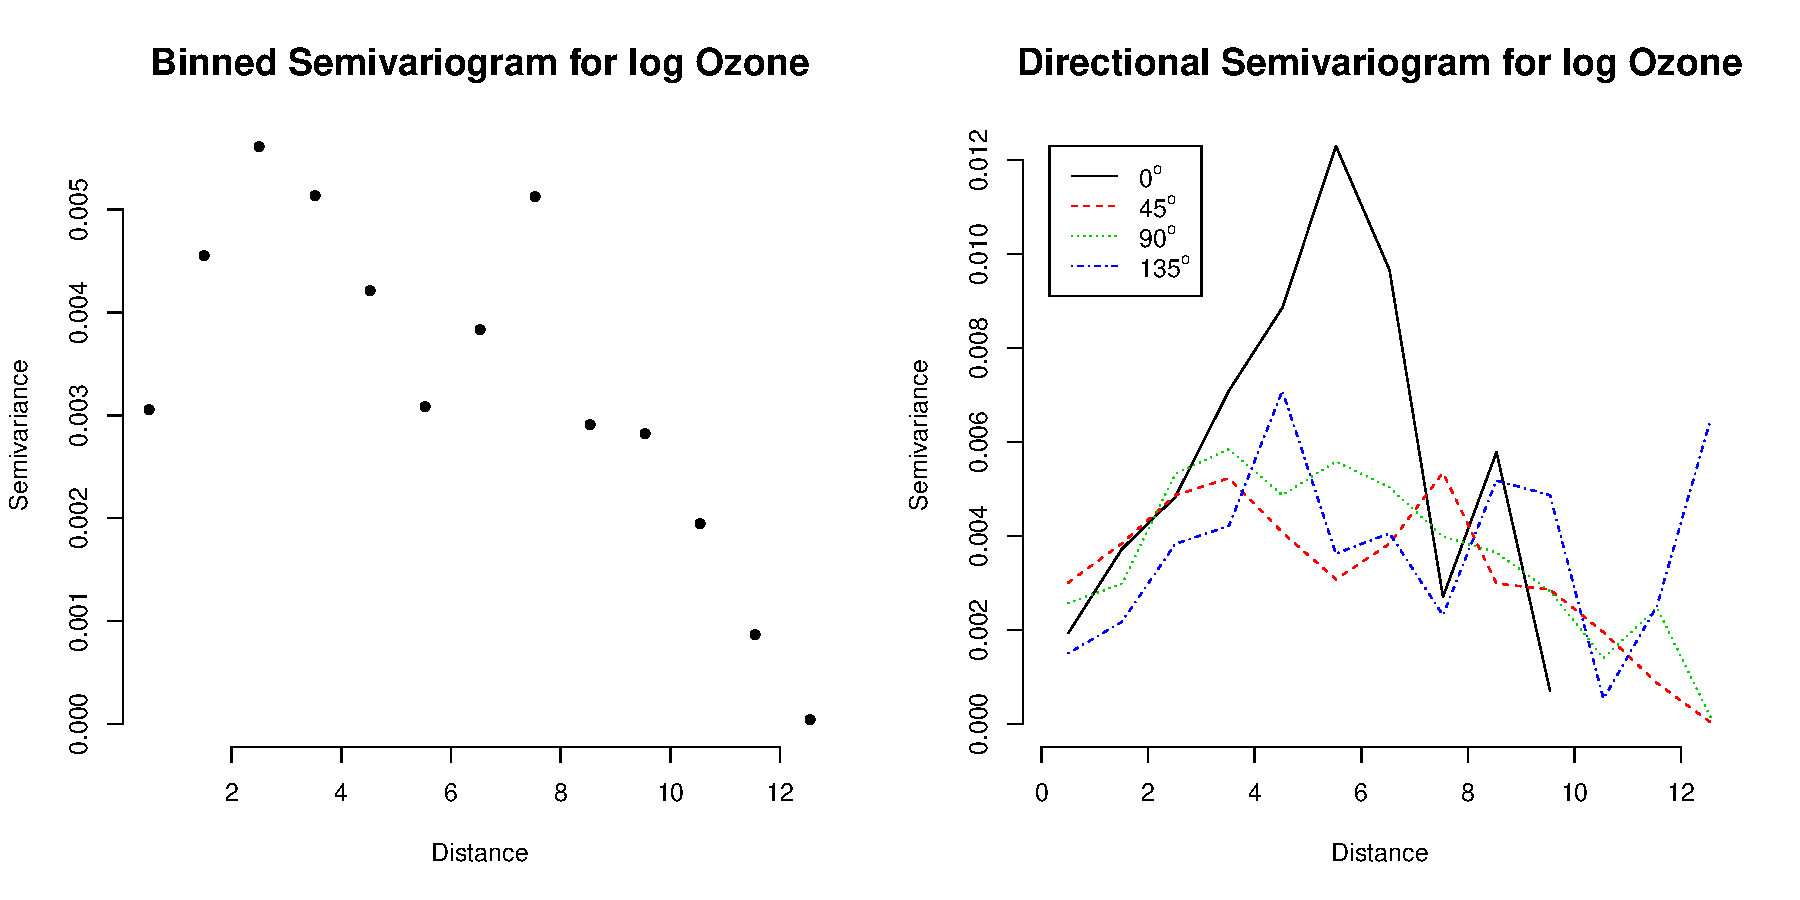
\includegraphics[scale=0.5]{figs/variogram.pdf}
\end{center}
\caption{Omnidirectional semivariogram (left) and directional semivariograms (right).}
\end{figure}

Some possible issues with this include how we are calculating our distances. We use euclidean distance on longitude and latitude, but this is likely to be a poor or inconsistent measurement of distance given the large geographic area within which we are working.
\bigskip

Another potential problem is that our omnidirectional semivariogram (left, Figure 3) seems to be decreasing. This could be because of a really small effective range, which is itself pretty disconcerting. A very small $\phi$ would essentially mean that there is little to no spatial correlation between observations.
\bigskip

We do a least squares fit to the omnidirectional semivariogram for parameters in the Mat{\'e}rn correlation. The function we are minimizing is
\[ f(u; \sigma^2,\phi) = \sum_{i=1}^n\left[\sigma^2 (1 - \rho(u_i, \phi, \nu)) - y_i\right]^2 \]
where $u_i$ is the distance obtain from the omnidirectional semivariogram, $y_i$ is the empirical semivariance, $\phi$ is the range, $\nu$ is the smoothness, $\rho$ is the Mat{\'e}rn correlation function, and $\sigma^2$ is related to the sill. We fix $\nu$ to be $0.5$, $1$, $1.5$, and $2.5$ and estimate the remaining parameters by maximizing $f$. The estimates for the parameters are shown in top right corners of the plots in Figure 4. From these, we do see a very small $\phi$.

\begin{figure}[ht]
\begin{center}
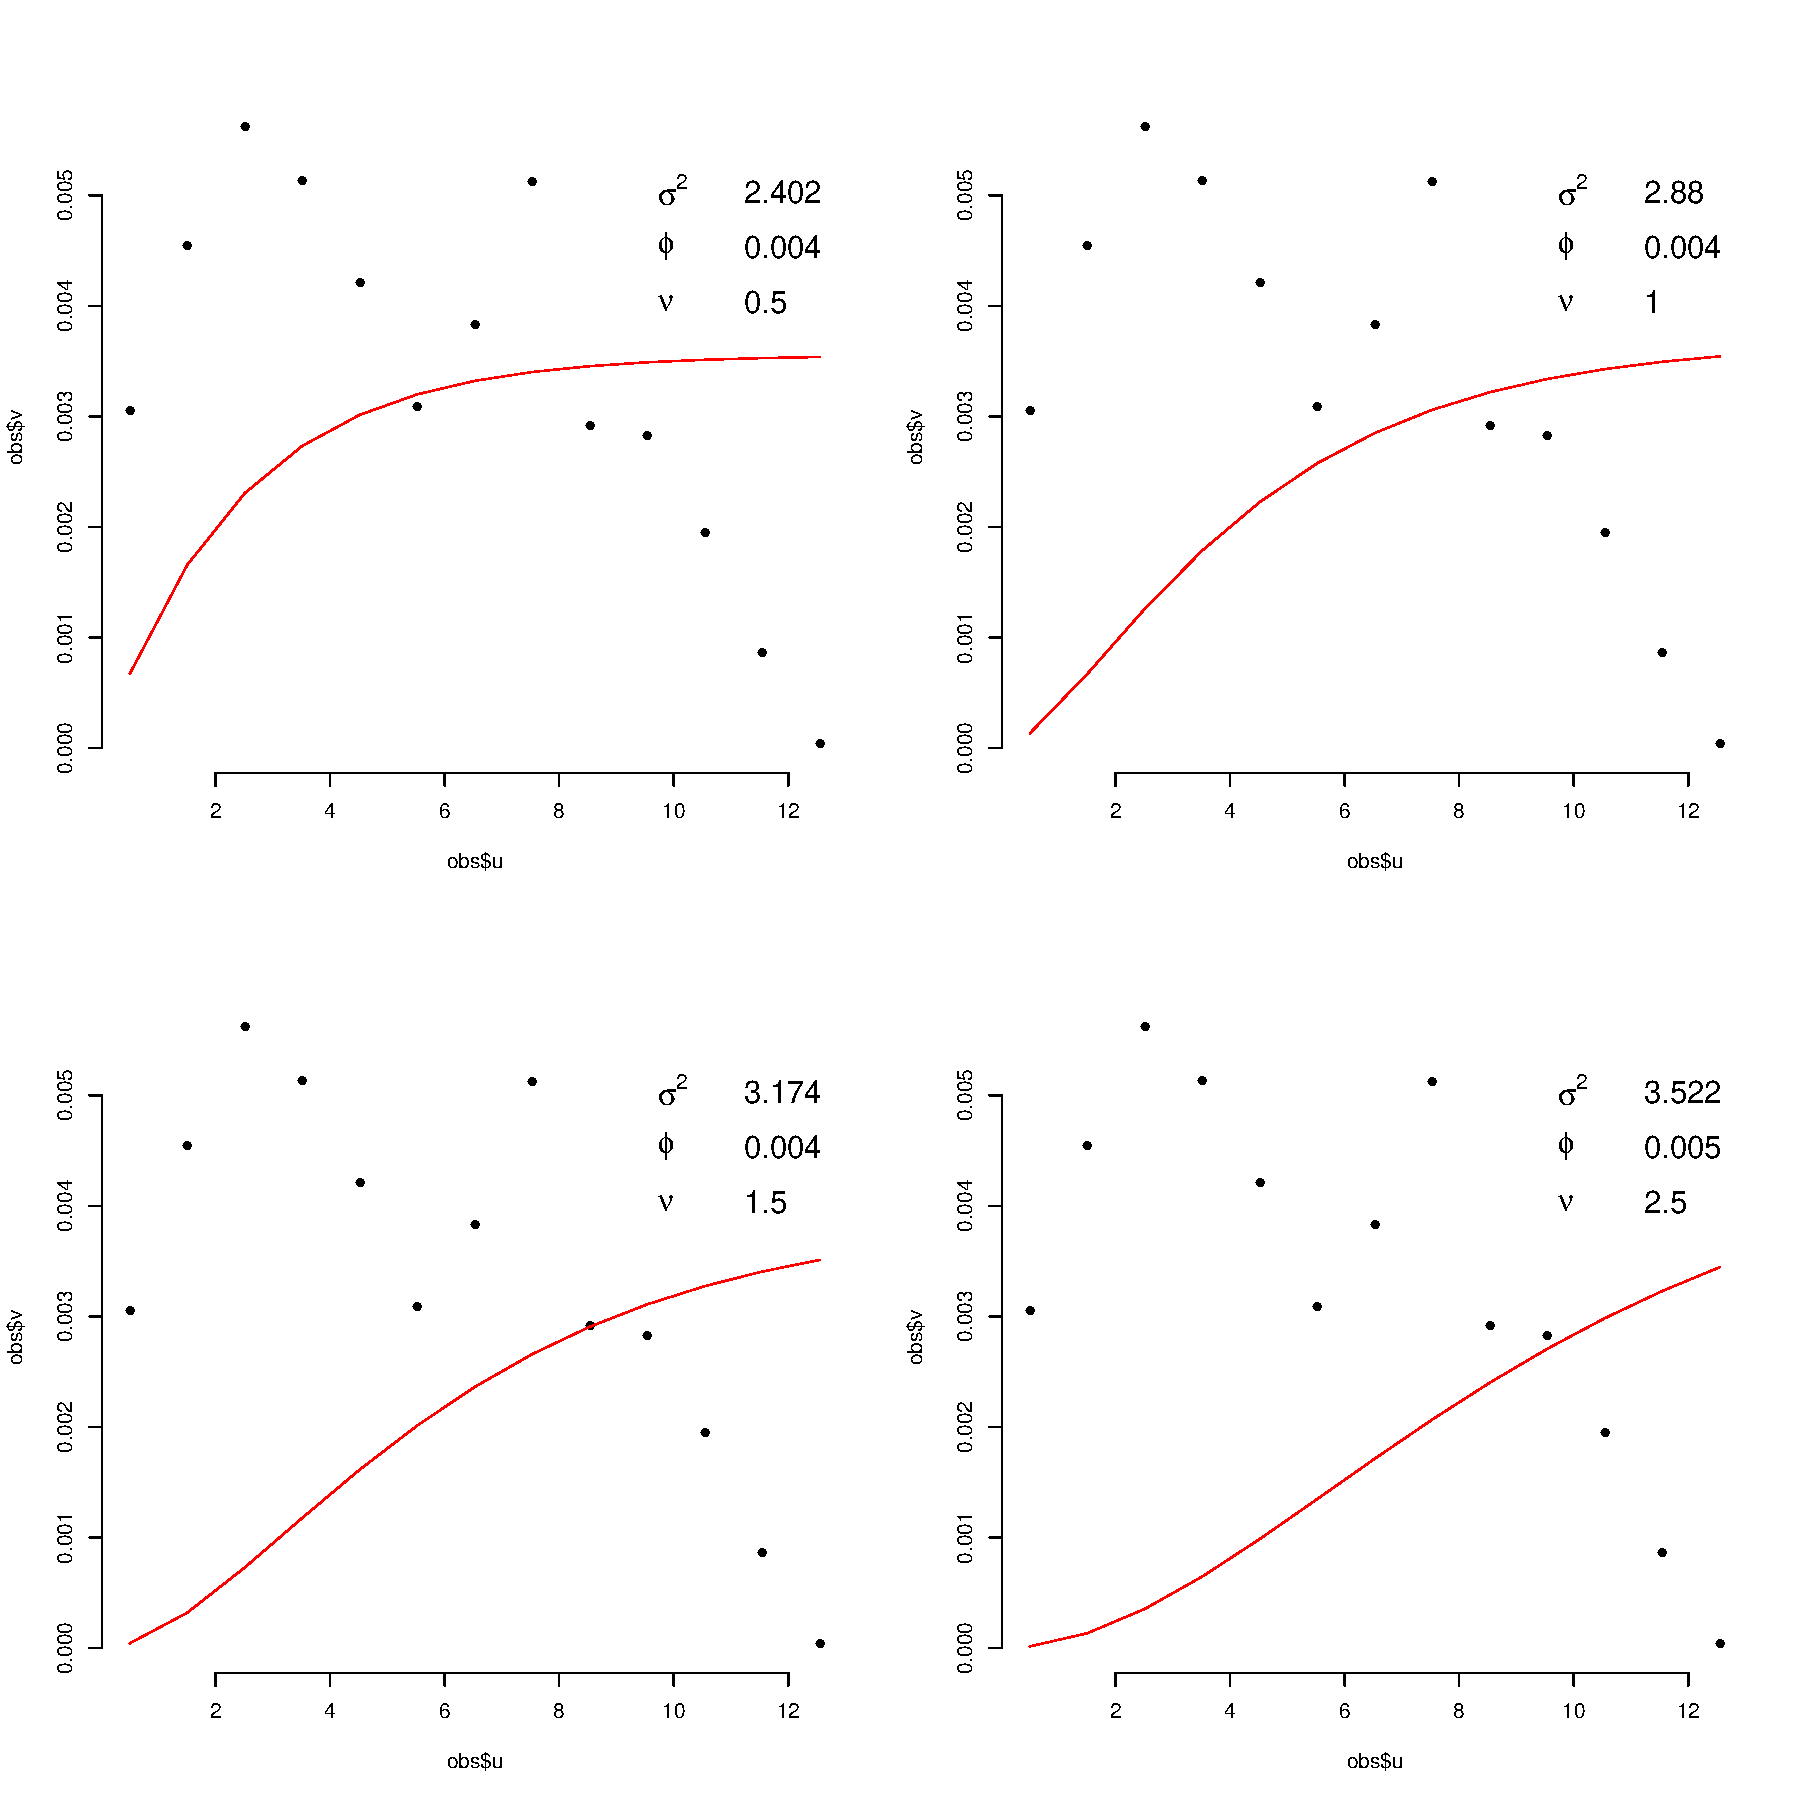
\includegraphics[scale=0.30]{figs/matern.pdf}
\end{center}
\caption{LSE for the Mat{\'e}rn correlation.}
\end{figure}

A nugget effect was not included because this lead to a $\phi=0$, which I didn't want. This was because I was insistent on fitting a GP, but with $\phi=0$ there is no need for a GP since all the covariances will be zero. That, or I spent a lot of time doing and understanding the wrong thing. Anyway.

\section{Model}

The model we fit is given by
\begin{align*}
X &= \mu + \epsilon,~~~~~\epsilon\sim N(0,\tau^2 I) \\
\mu &= D\beta + v,~~~~~v \sim N(0, \sigma^2 R(\psi))
\end{align*}
where $D=D(s)$ makes up the design matrix at each location $s\in S$. In our case, $D$ has a column of ones (intercept), the longitudes, latitudes, and interactions terms. The matrix $R(\psi)$ is computed using the Mat{\'e}rn correlation function. We are left with
\[ X \sim N(D\beta, \tau^2 I + \sigma^2 R(\psi)). \]
We let $\gamma^2=\tau^2/\sigma^2$, leading to 
\begin{align*}
X &\sim N(D\beta, \tau^2 (I + 1/\gamma^2 R(\psi))). \\
X &\sim N(D\beta, \tau^2 K(\psi)).
\end{align*}
where $\gamma^2$ is absorbed into the vector $\psi=(\phi, \nu, \gamma^2)$. For simplicity, we write $K(\psi)=K$.
\bigskip

The previous result leads to the following likelihood
\[ L(\beta, \tau^2, \psi) \propto |K|^{-1/2}(\tau^2)^{-n/2}\exp\left\{-\frac{1}{2\tau^2}(X-D\beta)^\top K^{-1}(X-D\beta)\right\}. \]

We obtain posterior samples using the blocking strategy described on pages 6 and 7 of the slides on Bayesian inference. From these, we have
\begin{align*}
\beta|\tau^2,\psi,X &\sim N(\hat{\beta}, \tau^2 D^\top K^{-1} D) \\
\tau^2|\psi,X &\sim IG(a + (n-k)/2, b + S^2/2) \\
p(\psi|X) &\propto |K|^{-1/2}|D^\top K^{-1} D|^{-1/2}(S^2+2b)^{-\frac{n-k}{2}-a}p(\psi) 
\end{align*}
where $\hat{\beta}$ is the solution to $D^\top K^{-1} D \beta = D^\top K^{-1} X$ and $S^2 = (X-D\hat{\beta})^\top K^{-1} (X - D\hat{\beta})$. I expect $\tau^2$ to be small, so I let $a = 3$ and $b = 2$, which provides an inverse gamma with finite mean and variance, centered around 1.
\bigskip

For $\psi$, we have $p(\psi)=p(\phi,\nu,\gamma^2)\propto p(\phi)p(\gamma^2)$, where $\nu$ is constrained to be one of the values in $\{0.5, 1, 1.5, 2.5, 3.5\}$. We let $\phi$ and $\gamma^2$ have gamma distributions each with mean and variance 1, as these are also expected to be small.

\section{Results}

\begin{table}[ht]
\begin{center}
\begin{tabular}{lrrr}
\hline\hline
 & \multicolumn{1}{l}{Mean}
 & \multicolumn{1}{l}{2.5\%}
 & \multicolumn{1}{l}{97.5\%} \\ \hline
$\beta_0$ &  8.212 & -45.068 & 63.040 \\
$\beta_1$ &  0.132 &  -0.595 &  0.875 \\
$\beta_2$ & -0.264 &  -1.549 &  0.991 \\
$\beta_3$ & -0.003 &  -0.020 &  0.014 \\
$\tau^2$   & 0.045 & 0.034 & 0.060 \\
$\phi$     & 2.937 & 0.956 & 6.277 \\
$\gamma^2$ & 1.736 & 0.195 & 4.916 \\
\hline\hline
\end{tabular}
\end{center}
\caption{Posterior parameter means and 95\% interval bounds.}
\end{table}

\begin{table}[ht]
\begin{center}
\begin{tabular}{lrrrrr}
\hline\hline
$\nu$ & 0.5 & 1 & 1.5 & 2.5 & 3.5 \\
Prob  & 0.002 & 0.036 & 0.116 & 0.321 & 0.522 \\
\hline\hline
\end{tabular}
\end{center}
\caption{Posterior probabilities (bottom) of $\nu$ being a specific value (top).}
\end{table}

full model DIC =  - 183.3267

\begin{figure}[ht]
\begin{center}
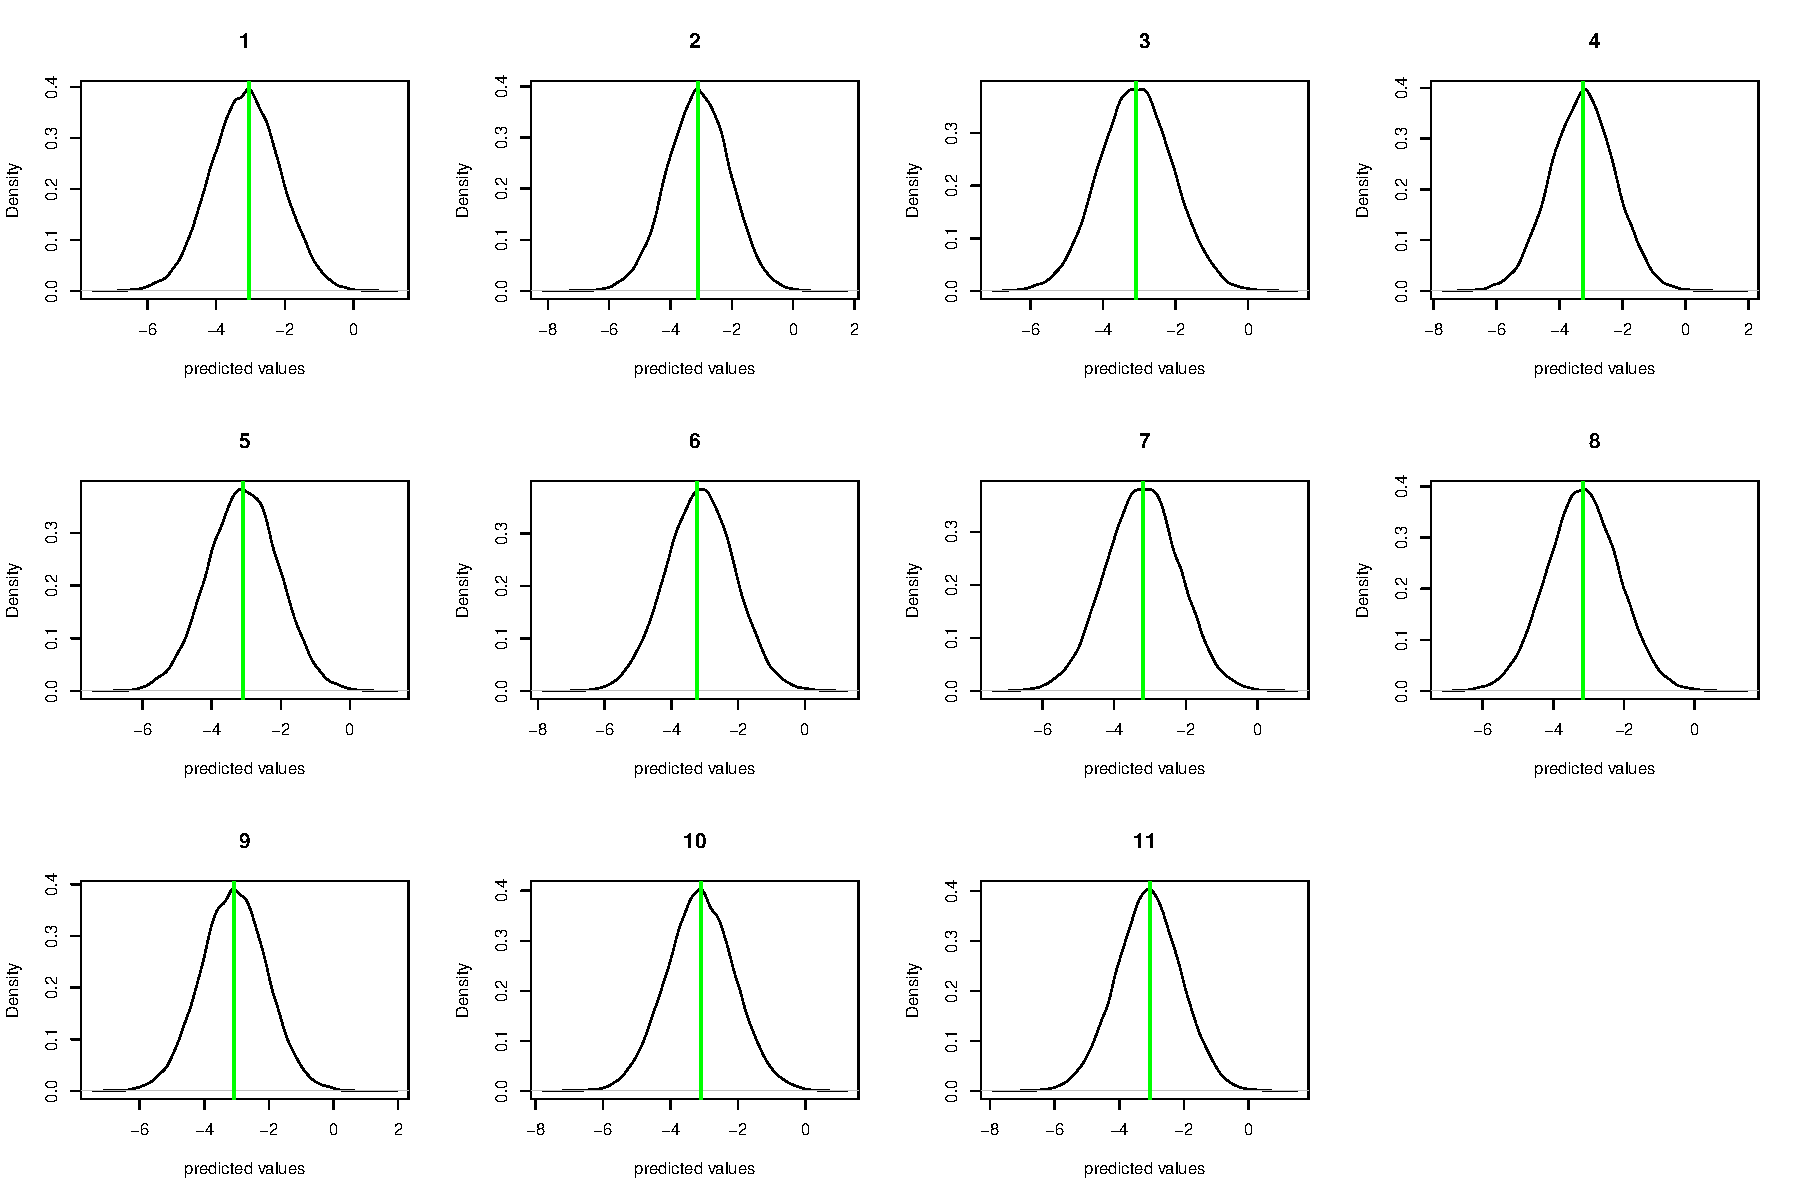
\includegraphics[scale=0.40]{figs/prediction.pdf}
\end{center}
\caption{Predictive distributions for the hold out sample.}
\end{figure}

\section{Conclusions}







\end{document}
